\documentclass[16pt]{beamer}
\usepackage{caption}
\usetheme{Madrid}
\usecolortheme{beaver}
\usefonttheme{serif}
%\pgfdeclareimage[height=1.3cm]{logo}{fig/logo}
%\logo{\pgfuseimage{logo}}
\usepackage[framemethod=TikZ]{mdframed}
\usepackage{bookman} % the used font
\usepackage{booktabs} % Allows the use of \toprule, \midrule and \bottomrule in tables
\usepackage{amsmath,amsfonts,mathrsfs,amsthm,amssymb,ctex,tikz,bm,graphicx,hyperref,geometry,listings}
\geometry{left=1cm,right=1cm}
\usepackage{gbt7714}
\lstset{
	frame=none,
	aboveskip=3mm,
	belowskip=3mm,
	showstringspaces=true,
	breaklines=true,
	columns=flexible,
	framerule=1pt,
	rulecolor=\color{gray},
	backgroundcolor=\color{white},
	basicstyle={\ttfamily},
	numbers=left,
	numbersep=1em,
	%stepnumber=5,
	numberstyle=\color{black},
	keywordstyle=\color{blue},
	commentstyle=\color{gray},
	stringstyle=\color{mauve},
	tabsize=3
}
\setbeamertemplate{caption}[numbered]

\title[标题]{标题}
\subtitle{答辩报告} % (optional)
\author[数学与统计学院]{author1 \inst{1} \and author2 \inst{1} \and author3 \inst{1}}
\institute[某大学]{\inst{1}信息与计算科学}
\date[\today] % (optional)
{\today}

\AtBeginSection[]
{
	\begin{frame}
		\frametitle{目录}
		\everymath{\displaystyle}
		\tableofcontents[currentsection]
	\end{frame}
}


\begin{document}
	\frame{\titlepage}
	
	\begin{frame}
	\frametitle{目录}
		\tableofcontents
	\end{frame}
	
\section{引言}
	\begin{frame}
		\frametitle{引言}
		\begin{itemize}
			\item \textbf{问题1:}这里输入文字
			\item \textbf{问题2:}这里输入文字
			\item \textbf{问题3:}这里输入文字
		\end{itemize}
	\end{frame}
	
\section{标题1}
	\begin{frame}
		\frametitle{第一部分}
		这里输入文字
	\end{frame}

	\begin{frame}
	\frametitle{第二部分}
	以下是\texttt{matlab}代码
	\lstinputlisting[language=matlab]{code/matlab-code-q1.m} 
	

	\end{frame}

\section{标题2}
\begin{frame}
	\frametitle{第一部分}

\end{frame}

\begin{frame}
	\frametitle{第二部分}
	这里输入文字\cite{ref}
\end{frame}

\section{标题3}
\begin{frame}
	\frametitle{第一部分}
	这里输入文字
\end{frame}

\begin{frame}
	\frametitle{第二部分}
	这里输入文字
\end{frame}

\section{最后}
	\begin{frame}
		\frametitle{最后}
		\begin{figure}[H]
			\centering
			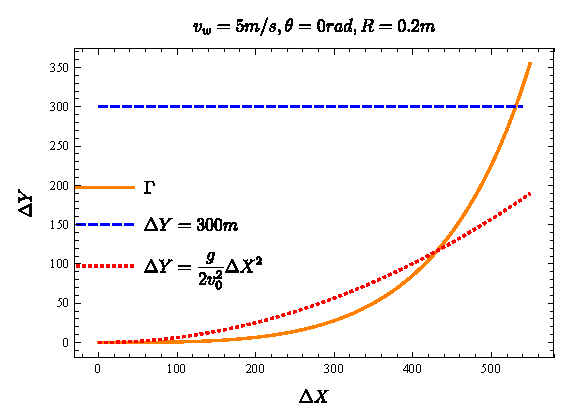
\includegraphics[width=0.6\linewidth]{figure/hlx-q1.eps}
			\caption{与理想状态下的对比图}
			\label{fig:hlx-q1}
		\end{figure}
	\end{frame}
	
	\begin{frame}
		\frametitle{第二部分}
	\end{frame}
	
\section{参考文献}
	\begin{frame}
		\frametitle{参考文献}
		\bibliography{ref/ref}
	\end{frame}
	\begin{frame}
		\Huge{\centerline{Thank you!}}
	\end{frame}
	
\end{document}